\chapter{Implementation}

%The implementation should look at any issues you encountered as you tried to implement your design. During the work, you might have found that elements of your design were unnecessary or overly complex; perhaps third party libraries were available that simplified some of the functions that you intended to implement. If things were easier in some areas, then how did you adapt your project to take account of your findings?

%It is more likely that things were more complex than you first thought. In particular, were there any problems or difficulties that you found during implementation that you had to address? Did such problems simply delay you or were they more significant? 

%You can conclude this section by reviewing the end of the implementation stage against the planned requirements. 

\section{Arithmetic}
The arithmetic construct was the first thing implemented.
It is a standalone piece of code only exposing a single method, Parse, which takes a string representing an equation and returning a tuple of the evaluated value and an error.
Because of this isolation I created it as a subpackage which also allowed me to simplify the error handling.

I was able to panic and recover\footnote{Panic is similar to an exception in other languages but has different semantics. Errors in Go should be passed through the use of multiple return values instead.} to completely unwind the parser and lexer.
Although panics are reserved for truly exceptional cases in Go, they had to be used in this case.
Errors encountered during lexing or parsing of a language are almost always fatal as they leave the system in an indeterminate state.
For example, the following make no sense in the context of a POSIX shell equation:
\begin{verbatim}
++
  or
35 67 89
\end{verbatim}
This is an implementation detail and can of course be treated differently.
In bash the '++' symbol can represent post-increment or pre-increment depending on its position.
The numbers could also be joined together into a single literal; Python and Java do something similar with underscores rather than spaces\cite{UNDERSCORE-NUM-LITERAL}.

One of Go's golden rules is 'never raise a panic across package boundaries' and to do this we defer\footnote{A Go construct that allows running a final function no matter how the function returns. the os.Exit is the only way to skip these.} a recover function.
If recover detects we have panicked it checks to see if it was a panic we created.
If it was then it is turned into an error and retuned normally. 
Runtime errors are allowed to crash the program.

During testing it was discovered that in the case of zero division the checks where not through enough the was allowed panic to bubble up rather than being converted into an informative error. 
The fix for this would be the addition of a division helper function similar to that used for shifting (See \ref{lst:arith-shift}) which would catch the runtime panic and raise a custom one that could be detected properly. XXX % Add reference to integration test that caught it.

\newpage %XXX NEWPAGE 
\subsection{Lexer}
The Lexer was completed during the first iteration as planned and has a good set of unit tests that where used to ensure the correctness of returned tokens.

The syntax for equations can consist of just variable names, symbols and numeric literals.

Variable names are detected using a state machine version of the following regular expression, \verb![a-zA-Z_][a-zA-Z0-9_]*!.

POSIX requires that detection of numeric values can be done in base 8 (Octal), 10 (Decimal) and 16 (Hexadecimal).
Values are always converted to base 10 for use inside the lexer.
If the literal is invalid, e.g \verb!0xffk! an error is returned that unwinds the parser.
The Scope struct (See~\ref{sec:scope}) does not yet have a way to perform transactions so any assignments that have already been conducted when an error occurs will persist.
Figure~\ref{fig:arith-assign-fail} shows that dash also does this and the spec does not mention how it should work.

\begin{figure}[hp]
    \centering
    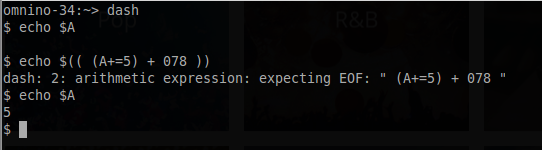
\includegraphics[width=0.8\textwidth]{arith-fail-with-assign.png}
    \caption[Dash assignment even with an error]{The text shown when the error occurs is very uninformative. bash does a slightly better job but still assigns to the variable.}
    \label{fig:arith-assign-fail}
\end{figure}

Symbols are the simplest thing to detect (See code in~\ref{lst:arith-symbol-lex}).
They only require one character of lookahead to be determined from any other symbol.
Some symbols also have an assignment variant.
If we encounter a symbol where this is possible, e.g '+',  a flag it set that will cause a check for a subsequent equal symbol.
If one is found the code takes advantage of the definition order of the tokens to change them to their equivalents.

\subsection{Parser}
The parser was not completed along with the lexer in the first iteration as had been planned.
It was finished in the second one along with extensions to Scope.

The tokens passed from the lexer are assigned to their node type by a simple switch statement.
These node types are used to abstract the functionality of similar operations.
For example $a + b$, $a * b$ and $a \mathrel{+}= b$, $a \mathrel{*}= b$ show that behaviour is similar and it is just the operation that differs in most cases .
Respectively they would be created as Infix and InfixAssign nodes with a value set to indicate what operation is desired.
Operations are functions that are stored in a hash tables for each type of node.

The Pratt parser requires that each node have two functions and one value, see~\ref{lst:arith-node-interface}.
Since Go interfaces can only consist of methods I just changed the value to a getter method instead.

\subsection{Variables}
To begin with I created stub methods on the parser that would eventually interact with the supplied scope.
When arithmetic was complete and I started work on the Scope these methods where changed to actually work.

Values are converted to strings before being stored.
If a retrieved variable can be parsed as octal, decimal or hex they are converted to base 10 before being returned and used.
If a variable cannot be parsed as a number or doesn't exist a value of zero is used instead.

Variables can only be accessed by using their unprefixed form, i.e \verb!(( a = 5 ))! will work, but \verb!(( $a = 5 ))! will not.
This is because variable expansion is a separate process and is done before arithmetic expansion.
Because of the flawed lexer design prefixed variables are not detected properly when used inside the construct and will cause an error (See~\ref{sec:main-lexer-arith}).

\subsection{Ternary}
The ternary operator is unique in that it operates on three values.

Unfortunately due to the fact that the tree is evaluated as it is constructed by my version of the pratt parser a bug surfaced.
When both sides of the environment contained assignment operators variables could be modified twice or always assigned the second value.
E.g With \verb!y = 0! an equation like \\ \verb!x ? y += 1 : y += 3! would make \verb!y == 4! no matter which side was meant to execute.

I left the bug with a failing test case while I continued the project.
I then went back to fix it in the last iteration using the knowledge I had gained during the project.

My fix \textit{feels} ugly and I am not completely happy with it despite the fact it works.
At each point of the ternary the position of the lexer is recorded and when the end of the equation has been de
\section{Scope}
\label{sec:scope}
The scope object was created during the second iteration alongside the arith parser.
It was also created as a subpackage because putting it in the main package was impossible since Go completely disallows circular references.

As is obvious from the package name, 'variables.Scope' and the headings in this section, the responsibilities of the class grew quickly and it quickly became mislabeled.
I realised the problems that had been created by the package layout
as I started to implement user functions in the penultimate iteration.
At this point it would have taken significant work to correct and the benefits would have been minimal.

\subsection{Variables}
The original Scope object was only used to get and set variables but it has lots of complexity.
It contains a list of hash tables which are searched in reverse order when setting, updating or retrieving anything.
The first value matching the name is used.

I created it this way as I knew that it would be needed by both commands with temporary assignments and functions using the local builtin.

Commands take a list of environment variables each as a string in the form, "VARNAME=FOO".
This meant that when I got to the stage when commands where being executed I had to add an Environ function to get them in the correct form.
The complexity of this function is O(2n), where n is the number of variables set in the shell, but I could not see a way to improve this without harming the performance of other aspects.

The design does not currently support variable flags.
This means that everything is exported to the environment of a new command.
Adding an export flag and a builtin function to set it would take little effort though.
Flags would also allow integer typed variables.
Changing the Variable struct to contain an isInteger bool and then when updating this variable use the result of 'arith.Parse(value)' instead of 'value'.

\subsection{User Functions}
\label{sec:user-functions}
User functions where added in the penultimate iteration.
The way they are stored in the Scope object shows how I was bitten by lack of forethought area of package layout.

\begin{verbatim}
type Scope struct {
	...
	Functions    map[string]interface{}
	...
}
\end{verbatim}

It shows that I have had to use a map of interface\{\} to store the NodeFunctions.
It is similar to a \verb!void *! in C as Go's implicit satisfaction of interfaces mean that everything satisfies the empty one.

This was done as storage and usage of a NodeFunction is done during the Eval phase which is defined in package main.
The solution would have been to create a subpackage for nodes.
However the work required to change the parser during the last week was greater than the bad practice of using interface\{\} here.

\subsection{Aliases}
Aliases where finished in the time frames.
They will however require storage in the Scope object and use of a builtin command to put them there.

The way the main lexer is created will also have to be different as aliases are expanded before anything is parsed but only when they are known about.

They also only take effect after after the compound block they are declared in is evaluated.
\begin{verbatim}
foofunc() {
    foo "IT WORKS"
}

alias foo=echo
foofunc
\end{verbatim}
This would cause the shell to print an error as the alias did not exist before the function was parsed.
foo will be available for the rest of the script but the foofunc function will always cause an error.

\section{Main Lexer}
The main lexer is a coroutine based Non-Deterministic Finite Automata(NDFA).
I was inspired to use this design by Rob Pike's presentation of Go's template parser\cite{PIKE-LEXING-VIDEO}.
The code in the standard library is quite simple and is easy to follow along with.

A concurrent run loop is started when the lexer is created which means that when run on machines with multiple cores (Almost everything modern) performance will be slightly improved.
During this run loop state functions are called, beginning with lexStart, which either return another state function or nil to indicate that lexing has completed. 
Each state defers to others when possible to reduce code duplication.

Given the text \verb!"abc $def"!. lexStart will pass control to the lexDoubleQuote function when it see's the '"' character which will pass control to the lexSubstitution when it see's '\$'.
This will determine that lexSimpleVariable is needed as neither '\{' or '(' follow the dollar sign.
Once that completes control is returned to lexDoubleQuote which will see the closing quote, emit a TokenWord which contains the contents of the string, and finally return control to lexStart.

The emit function takes a token type and constructs a lexitem, sometime know as a lexeme, that contains the required information to be parsed and evaluated successfully.
This information includes the line number and position of the token in the source, its string representation, if the string should be treated as quoted and substitution structs.
Substitution structs hold information on how to replace interpolated values, See~\ref{sec:substitution}.
The values in the lexer that hold this information are reset when an emit occurs.

For a simpler syntax this design is perfect but it turned out to be unsuited to the shell.
They are some times in the next section when creating a new lexer and using its output is mentioned.
Because of the concurrent nature of the lexer this is the only way to safely get tokens while in the middle of lexing another portion of the input.
This workaround may also suffer from memory leaks as there is a reference to the lexer in the go-routine thread which might prevent the garbage collector from collecting it.

Tokens returned from the lexer are one of three types.

Word tokens which are strings or unquoted text not recognized as a keyword.

Control tokens which represent keywords such as 'for'.
Detection of these tokens is disabled by the parser in certain cases.
For example the following is allowed \verb!for for in for; do for=for; done; echo $for! as both the second and third for are parsed with the flag to disable keyword detection.

The final types are operators like EOF and Newline. 
Newlines can also be suppressed during the lexing which will then continue until a non Newline token is found. 

\subsection{Words}
The word lexing code was completed during the third iteration along with the stubbed parser.

Words are any text that is not a control operator, symbol or substitution.
They contain a field that allows the parser to check if it is a string.
This information will eventually be used to determine the expansions and word splits to perform on it.

\subsubsection{Strings}
Two functions are used for strings as the shells has both raw quotes and interpreted quotes.

Raw quotes use the single quote character and are very simple.
Every character is copied as is except the EOF and the matching single quote.
EOF causes an unterminated string error.
The end quote causes the string to be emitted.

Interpreted strings, which use double quotes, should allow variables, both types of subshells and escape sequences.
Unfortunately escape sequences where not completed so the string '\\n' will be treated as two separate character rather than a newline.
The position of subshells and variables in a string are indicated by the SentinalSubstitution character.
The subs list of each lexitem holds the structures that can be called to replace these sentinals.
This is done to abstract to complexities of substitutions.
Interpreted strings also throw an error when encountering EOF.

When they where created during the third iteration both single and double quotes behaved as raw strings.
As the capabilities of the lexer improved the lexDoubleQuote function could add a new rule to its switch statement and pass control to incorporate them.

\subsection{Variables}
Variables where completed in two stages.
Simple ones in the fourth iteration alongside extensions to the parser.
Complex variables during the XXX.

The lexer has a lot of knowledge about variables due to the concurrent design and the interpreted nature of strings.
This would be better suited in the parser and it would also fix the problems that exist with more complex substitutions.
A complex variable substitution of the form \verb!${foo:-$bar}! does not currently work.

This shows a variable 'foo' being operated on by the ':-' operator.
When I created the lexComplexVariable function I used a naive lexer for anything after the operator with the intention of replacing it.
It gathers everything as is upto the next '\}' character and uses it as the value.
Creating another lexer using the remaining input and extracting tokens would be the solution in the current state.
However redesigning the lexer to be recursive descent would make it even easier.

\subsubsection{Variable Lexing Bug.}
While writing this section and inspecting the code I noticed that the naive collection does not check for the EOF character.
This means that a memory based DOS attack is possible by just using a file with the contents \verb!${a-!.
The lexing code will continue appending the EOF character to the buffer as calls to 'next' continuously return it once it has been reached.

The previously mentioned design improvements would have removed this bug.
A fix in the meantime would be to simply panic if the EOF character is seen.
An unterminated variable is not defined behaviour and while a panic will not be the most descriptive way of indicating the error it would stop resource abuse.

\subsection{Subshells}
The original form uses grave quotes as delimiters and the 'modern' version uses '\$( command )'.
They work similarly to user defined functions but output is captured instead of being output to the terminal.
Changes to the environment that take place inside a subshell are not propagated. 

For the modern version when the start of a subshell is detected a new lexer and parser pair is created with the remaining input.
This parser is started with IgnoreNewlines option and returns an AST of everything contained in the the brackets.
The lexer on the current level then adjusts its position in the input to the character after the closing bracket.
This works quite well but the same thing cannot be used for the old style.

\begin{verbatim}
$( foo $( bar $( baz ) ) )    # Modern

`foo \` bar \\\`baz\\\` \` `  # Old
\end{verbatim}
The code above shows how nesting three levels works using both type of subshell.
Parsing an old style subshell first requires that you find the correct ending grave, I.e not escaped or in a string.
Then you have to scan through the string and for every grave that is not quoted remove a level of nesting.
The first level uses a single backslash to escape and each subsequent level uses an additional two.
The result of this modification can then be passed into a new parser and the process repeated.

Once parsed both styles are represented identically in the AST.
Because of this I focused on implementing the modern style as the proof of concept.
The first attempt consisted of using the current parser, saving every piece of information the lexer stored and starting a second run loop.
This completely failed as both run loops contended over the item channel resulting in races.

The second attempt was the current and final design.
It originally had an intermittent race as it accessed the sublexers position and lineno values directly which where not always set correctly.
To fix this the 'nextLexItem' function was used to retrieve a token which would contain the correct position information.

\subsection{Arithmetic} \label{sec:main-lexer-arith}
As the heavy lifting is done by its own lexer and parser we only have to gather the contents to pass along.
The main lexer gained the ability to recognize them during the forth iteration along with simple variables.

This is done by counting the number of parentheses that are encountered while stepping though the input.
Lexing finishes when two consecutive right brackets that are part of a bracketed expression are seen.
I.e \verb!$(( 2+4 ) ) ))! will lex identically to \verb!$(( 2 + 4 ))! as right brackets are ignored when they are not consecutive or part of an expression.
Everything between the two markers is stored in a substitution object to be passed to 'arith.Parse'.

In the specification substitutions contained within this construct are expanded before itself.
E.g \verb!$(( 2 + $(echo 4) ))! should reduce to \verb!$(( 2 + 4 ))! and then be evaluated as math.
Again this was not completed because of the non re-entrant nature of the lexer. XXX













\section{Main Parser, AST \& Nodes}
The parser turns the tokens into nodes and constructs AST's with them.
It was developed iteratively as nodes and elements of the lexer where completed. 

Almost every node has a default exit status of success.
This is helpful as statements that dont run because their conditions evaluated false are showing correct behaviour.

Nodes also contain a number of other nodes depending on what they represent.
Terminal nodes such as NodeCommand, NodeEOF and NodeNoop are what other commands reduce too and don't contain further nodes.

The use of a node interface allows the behaviour of every node to be separated.
This is contrary to the design of dash which uses global state and a single function to dispatch to other evaluation functions.
This can be extremely confusing as it contains 7 GOTO statements and 6 blocks of conditional defines in only 128 lines (See~\ref{lst:dash-evaltree}).


\subsection{Simple Command}
A simple command is a line that contains a command with optional arguments and variable assignments.
The command can be a builtin (See~\ref{sec:builtins}), a function (See~\ref{sec:user-functions}) or an external command.
Simple commands are stored as NodeCommand's which incorporate the logic of decided what type of command to run as well as expanding the arguments and any variable assignments.
If the line with assignments also has an external command call, the assignments are temporary and are removed when the command completes.

During the third iteration this was created to support commands with arguments.
It was expanded during the fourth to accommodate variables assignments and during the fifth, for arguments that contained substitutions.
The simple command function is also the place that function definitions are detected and this was added during the penultimate iteration.

\subsection{Command}
Command is the function that parses the command structures of the code.
This includes the 'if', 'for', 'until', 'while' and 'case' expressions.
The code for parsing these is separated from the main function as they can be quite long.
One of the longest functions in the codebase is the parsing routine for a case statement and by splitting these up it allows you to focus on one thing at a time.

Each type of command has its own node that handles the details of its execution.
The NodeFor, NodeWhile and NodeUntil will have to understand the break and continue commands once they have been implemented.

Along with the commands that people expect this is also the place that command grouping occurs.
This feature is often seen when defining shell functions and some people may believe that, like in other languages, it is a part of their definition syntax.
However it can be used anywhere a command can including in a pipeline or in a conditional to avoid certain bugs.
A command group begins with a '\{' and ends with a corresponding '\}'.
Anything contained between the two is parsed as a separate group which allows redirections to be applied to everything it contains.
See the code in~\ref{lst:command-grouping} for examples.

\subsection{Pipeline}
The pipeline is a list of commands that will join their inputs and outputs to each other and then be run in parallel.

This allows simple utilities to be combined to produce complex transformations.
Since they are conducted in memory buffers overhead can be reduced by such an amount that they can be faster than common distributed computing tools like Hadoop\cite{AdamD45:online}.
Pipelines also encourage the Unix philosophies of programs that 'Do one thing and do it well' and 'Handle text streams; the universal interface'.
Observing this can help users solve problems with almost no programming\cite{LITERATE-VS-SHELL}.

The pipeline function also handles negation of the exit code.
Any Command or pipe prefixed with a '!' returns the opposite of its exit code, for 0 the return becomes 1, for any other value it becomes 0.

\subsection{And Or}


\subsection{List}














\section{Expansion}
Expansions are performed throughout the code to different degrees.
Some places dont require all of the possible expansions and explicitly pass flags to disable them.
This is a change from the C expansion code where the use of bitflags for every call was required.
I decided that the change was needed as it is rare to not want and expansion and it is easier to understand the logic of
'NoExpandTilde' than a series of or'ed flags.

Expansions are evaluated every time they are reached because of their 'impure' nature.

\subsection{Tilde}
When a tilde occurs either as the first character of a word or immediately following a ':' in a word it should be expanded.
The '\textasciitilde' can also be followed by text to indicate it should expand to the home directory of another system user.
Some shells have extended support for this and allow setting 'named directories' that can be expanded in the same way.

Support for this in the shell is basic.
If the first character is a tilde it is replaced by the path of the current users home directory.
The location of this directory comes from the 'os/user' package which wraps the platform dependant code needed to get this.
POSIX requires that the 'HOME' variable is checked before a lookup is conducted but the shell does not currently do this.

\subsection{Substitutions}
\label{sec:substitution}
Substitutions affect variables, commands and arithmetic.
Currently only commands can contain embedded substitutions but in the future all three will be able to nest each other.
This nesting means that it is possible to reach

XXX
\subsection{Globbing}
Globbing is the act of expanding the shells simple builtin pattern matching language to a list of files.
This look similar to regex syntax but isnt.
'*' can match any amount of any character, '?' any single character, and '[a-z]' a single character from the range.

By default glob looks in the current directory for files matching the provided pattern.
However if the pattern starts with a path that is the directory that will be searched.

I did not find a fnmatch function when I searched Go's documentation as so began looking online.
I eventually came across a years old gist that I forked, updated and used for this task.
It was only later that I realised that Go does provide the functionality I was looking for in the 'path/filepath' package.
Since the fnmatch library is only used in a few places and it is a single function call it offers no benefit over using the standard library function and should be swapped at the first opportunity. 

\subsection{Word Splitting}
Word splitting uses the value of a variable called the Internal Field Separator(IFS) to split expansions into multiple words.
The default value of this variable is ' \\n\\t' which splits on spaces, tabs and newlines.
While this may seem sensible it can lead to confusing behaviour and it is commonly changed to '\\n\\t'
for a so called strict mode.

This usually only occurs when variable and command substitutions are unquoted but some variables are special and have different behaviour.
E.g When the '\$*' variable occurs quoted it uses the first character of IFS to join the shells positional parameter into a single string.
\begin{verbatim}
IFS='-'
set - a b c
echo $@    # "a" "b" "c"
echo $*    # "a" "b" "c"
echo "$@"  # "a" "b" "c"
echo "$*"  # "a-b-c"
\end{verbatim}

Gosh does not perform word splitting of any kind.
This is probably the biggest problem with the implementation as it is required for correctly passing arguments to commands.
It is also used with special variables and in argument lists of functions and for loops.





\section{Builtin Commands}
\label{sec:builtins}
Builtin commands are used for two reasons, they either modify internal state and as such cannot be replaced by external commands or they are used often enough that the startup overhead of the executables being called could affect performance.

In the last iteration some of the most needed built-in commands were implemented.
These where 'cd' and 'local'.
The spec requires that these commands take some options 

I also implemented the 'true' and 'false' commands for performance reasons.
While these will not be bottlenecks in any program they show that commands can be easily created.
The biggest boosts will probably come from implementing 'echo' and 'printf' as these are commonly used commands.

As these commands are logically separate from the functionality of the shell I created a subpackage for them.
This again showed that package planning had not been considered well.
Both IOContainer and ExitStatus had to be moved from 'package main' to a subpackage.
This package has ended up with the nondescript name of 'package T' as it has no purpose other than to be a temporary home to these types.

XXX

\section{Circular References}
\label{sec:circular-refs}
Circular imports have been a problem during the project, see~\ref{sec:user-functions} and~\ref{sec:builtins}.
My experience with Go has never been with a project large enough to require subpackages and this was the main reason behind my lack of planning for them.
While it would have been possible to create everything in the main package this would have have left it quite crowded.
It is also had for a new person to understand what is important if things are not separated properly.
I experienced this while trying to learn from the source code of bash and dash.

A better design would have been to create a package each for the nodes, substitutions and the main lexer \& parser.
The only thing that would be in the main package would be the entrypoint function, in 'main.go', that sets up the run loop of parsing and evaluation.

XXX: